\documentclass{article}
\usepackage{fancyhdr}
\usepackage[margin=1in]{geometry}
\usepackage{amsmath}
\usepackage{amsfonts}
\usepackage{graphicx}
\usepackage{subcaption}
\usepackage{algorithmicx}
\usepackage[noend]{algpseudocode}
\usepackage{algorithm}
\usepackage{subcaption}
\usepackage{amsthm}
\usepackage{mathtools}

\usepackage{hyperref}
\hypersetup{colorlinks=true,
    linkcolor=blue,
    filecolor=magenta,
    urlcolor=cyan,}

\newcommand{\polyred}{\leq_{\mathrm{p}}}
\newcommand{\polyeq}{\equiv_{\mathrm{p}}}
\newcommand{\sprev}{S_{\mathrm{prev}}}

\DeclarePairedDelimiter{\ceil}{\lceil}{\rceil}
\newtheorem*{claim*}{Claim}

\pagestyle{fancy}
\lhead{CS 201: Operating Systems \\ \textbf{Instructor}: Jason Hibbeler \\ \textit{Discrete Event Simulator}}
\rhead{UVM, Fall 2018 \\ \textbf{Name}: Daniel Berenberg \\ \textit{Final Deliverable}}
%------------------------ header ------------------------------------------------------- 
\begin{document}
%---------------------------------------------------------------------------------------
\section*{Introduction}
Operating systems are complex software programs that allow users to safely interface with a computer
and perform various tasks. 
While most operating system are composed of millions of lines of code
with thousands of hours of development and thought behind their designs, 
it is possible to construct a simple software model called a discrete event simulator
that abstracts the behavior of an operating system's process management methodology 
and provides a sandbox for investigating operating systems related concepts (such as CPU scheduling) 
without worrying about the complexity of the software itself or the specifics of different types of processes.
\par
In the discrete event simulator model, processes with randomly distributed 
CPU and I/O burst times move between ready, running, and I/O blocked states in the form of discrete events. 
Discrete events encapsulate ``important'' (with respect to the OS behavior) moments
in a processes' lifetime. Events are chracterized in 6 different flavors 
(process submitted, process terminated, I/O request, I/O complete, and time slice expired) occurring at 
various time steps during the course of the simulation. 
For a given event, its associated process' parameters will be updated accordingly and 
cause the process to move between ready, running, and I/O blocked states.
\par
This document serves to profile the performance of the classical round robin CPU scheduling
algorithm and compare it against an artificial intelligence guided process management scheme
that seeks to learn adaptive scheme for time quantum assignment.
%---------------------------------------------------------------------------------------
\section*{System Description}
Here we describe the way the software model is designed and provide more detail to the 
algorithms behind round robin and adaptive preemption schedulign schema.
\subsection*{Software Hierarchy}
The discrete event simulator software is an object oriented implementation consisting of 
several interacting portions:
\begin{itemize}
    \item{\textbf{Process} is the ``currency'' of the system. Processes are instantiated with specific
          parameters (CPU and I/O burst times, CPU demand, arrival time, etc) and traded throughout the previously
          mentioned ready, running, and blocked states until either the simulation completes or the process' total demand
          reaches zero.}
    \item{\textbf{Event} are points in a Process' lifetime that are important to the OS\@. 
          Events point to a specific process at a certain timestep and inform the system how to react.} 
      \item{\textbf{CPU} is an object that accumulates its activity (context switch, idle time, active time) throughout 
          the simulation. CPUs also enable the functionality of allocating a processs and executing it for a certain duration,
          either until the process terminates, reaches an I/O fault, or its time quatum expires.}    
    \item{\textbf{DiscreteEventSimulator} guides the entire system. The largest portion of the DiscreteEventSimulator codebase
         consists of 6 conditions that, given an event, allow that event to be handled and trigger the creation of a new subsequent
         event.}
    \item{\textbf{ProcessFactory} is not part of the model whatsoever, but rather provides an elegant solution to on-the-fly
        process creation.}
\end{itemize}
\subsection*{Round robin scheduling}
Round robin scheduling assigns time quantum $Q$ to each process that enters the system. 
Processes are placed onto a ready queue and wait to be allocated to a CPU where they will
run for at most $Q$ timesteps before terminating, reaching an I/O fault, or are kicked off 
the CPU for the next process. 
The key to round robin scheduling for the purpose of this project is that each process
is assigned \textbf{the same} time quantum as it enters the system.
\subsection*{Adaptive process control}
Reinforcment Learning (RL) is a subset of machine learning algorithms that enable \textbf{agents} (schedulers) to occupy
and explore an \textbf{environment} (the operating system model). 
Agents are informed by their surroundings in the form of states $S$, actions $A$, and rewards $R$.
Upon taking action $A$ in $S$, the agent will travel to state $S'$ and recieve reward $R$.
The agent then updates its understanding of the environment accordingly based on $R$ and the
features of $S$ and $S'$.
\par
Supervised learning involves approximating a function input data $X$ to labels $y$. 
The RL framework's objective is to learn a function of states and actions $Q(s,a)$ that outputs an
approximation of the reward function upon taking $a$ at $s$. This learned function $\hat{Q}(s,a)$
provides a policy of behavior for the agent to act on.
\par
The adaptive proces control for this project is formulated by considering events in the simulation
as states, and the integers defined in $[1,200]$ as actions. The reward function is defined as the  
negative of the sum of CPU idle times between the last two events. The agent is informed by
various state attributes including the current time step, the total CPU demand left of the event's
process, the last quantum assigned, the time spent waiting in the system, and the time the 
process has spent in the system entirely; the approximate function $\hat{Q}(s,a)$ is given by the 
dot product of these features with a vector of learned weights $W$ $\hat{Q}(s,a)=\sum_{i}f_i(s)w_i$ that assert the precedent
of each feature, where $w_i \in W$ and $f_i$ is the $i^th$ feature of the state $s$ feature vector. 
Weights are updated based on the difference in the reward recieved and the approximated value upon entering the next state. 
%---------------------------------------------------------------------------------------
\section*{Experimental Design}
The experiments conducted are concerned with profiling the behavior of the two scheduling criteria
for different types of systems. The invariant parameter regimes of the system were chosen as follows:
\begin{itemize}
    \item \textbf{Simulation length} is 500,000 timesteps.
    \item \textbf{Context switch time} penalty was set to 1 timestep.
    \item \textbf{Process types} were the \texttt{batch} and \texttt{interactive} regimes provided.
\end{itemize}
Round robin constant quanta tested were quantums between 0 and 200 in steps of 5. In each case
of the adaptive preemption method and constant quanta, the methods were realized over the
15 independent simulations and tested on systems of 1 and 3 CPUs. 
%---------------------------------------------------------------------------------------
\section*{Results}
The results to the above described experiments are promising indicators that the adaptive
preemption framework is able to not only learn about them system and act accordingly,
but perform on par with, if not better than, many of the constant quanta used in
round robin scheduling.\par
Figure~(\ref{fig:params_per_q}) shows process statistics for each quantum. Each of the 15 simulations
is aggregated and averaged in order to generate this visualization. As shown, the figure indicates that
indeed the adaptive CPU scheduler either outperforms or has on par performance with round robin scheduling,
however the turnaround times for a 3 CPU system cannot be beaten by the RL agent. This can be attributed
to the fact that the process types used may not provide a ``difficult enough'' task for 3 CPUs, meaning
there isn't a strong factor of resource scarcity. In this regard, intuitively it makes sense that the
RL approximator may poorly fit the task.
\begin{figure}
    \centering
    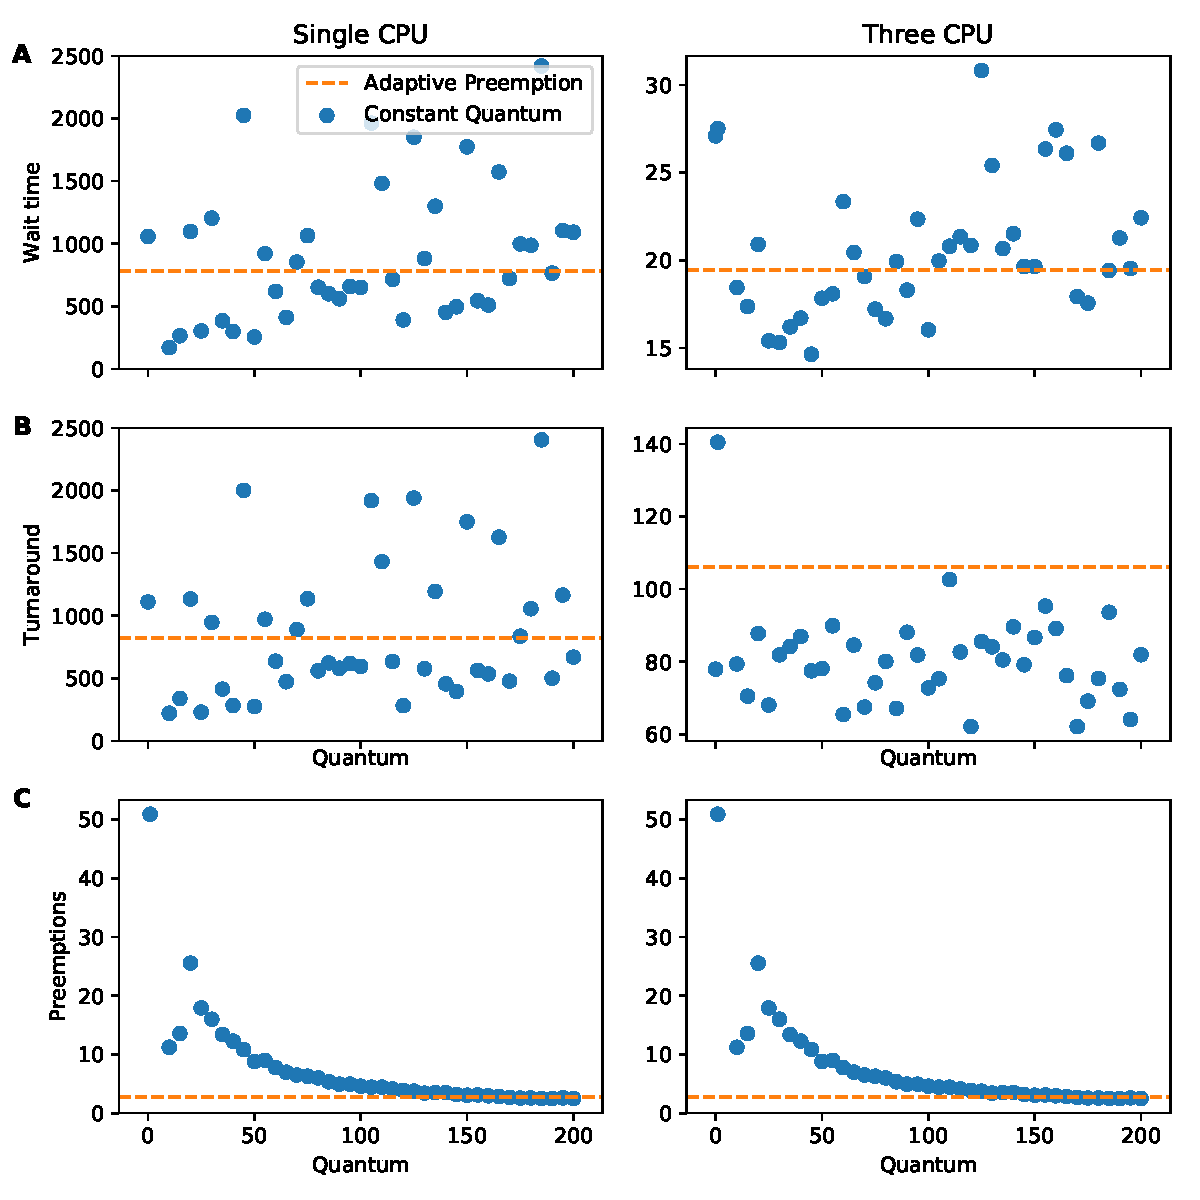
\includegraphics[width=0.75\textwidth]{figs/params_per_q.pdf}
    \caption{Process statistics per quantum. Panel \textbf{A} shows the mean wait time (time spent in ready queue) 
             of the final 1000 processes that terminated in the system for both single and tri-CPU systems.
             Panel \textbf{B} similarly shows the average turnaround times (time spent in system total).
             Finally, Panel \textbf{C} visualizes the average number of preemptions experienced per process per quantum.}
    \label{fig:params_per_q}
\end{figure}
\par
Figure~(\ref{fig:procs_completed}) provides further evidence of the on par behavior of the adaptive preemptor to
the round robin scheduler. As shown, the panel \textbf{A} relates that the RL agent is able to acheive at least the
average performance of round robin across all quantums for each CPU count variant. Meanwhile, panel \textbf{B} shows
that in all cases, be it with or without a high number of CPUs and regardless of time quanta, the system is flooded with
processes in the beginning causing long term process time debt for the course of the simulation. 
Functionally this means slowing down the throughput (processes completed per $t$) of each process type.
\begin{figure}
    \centering
    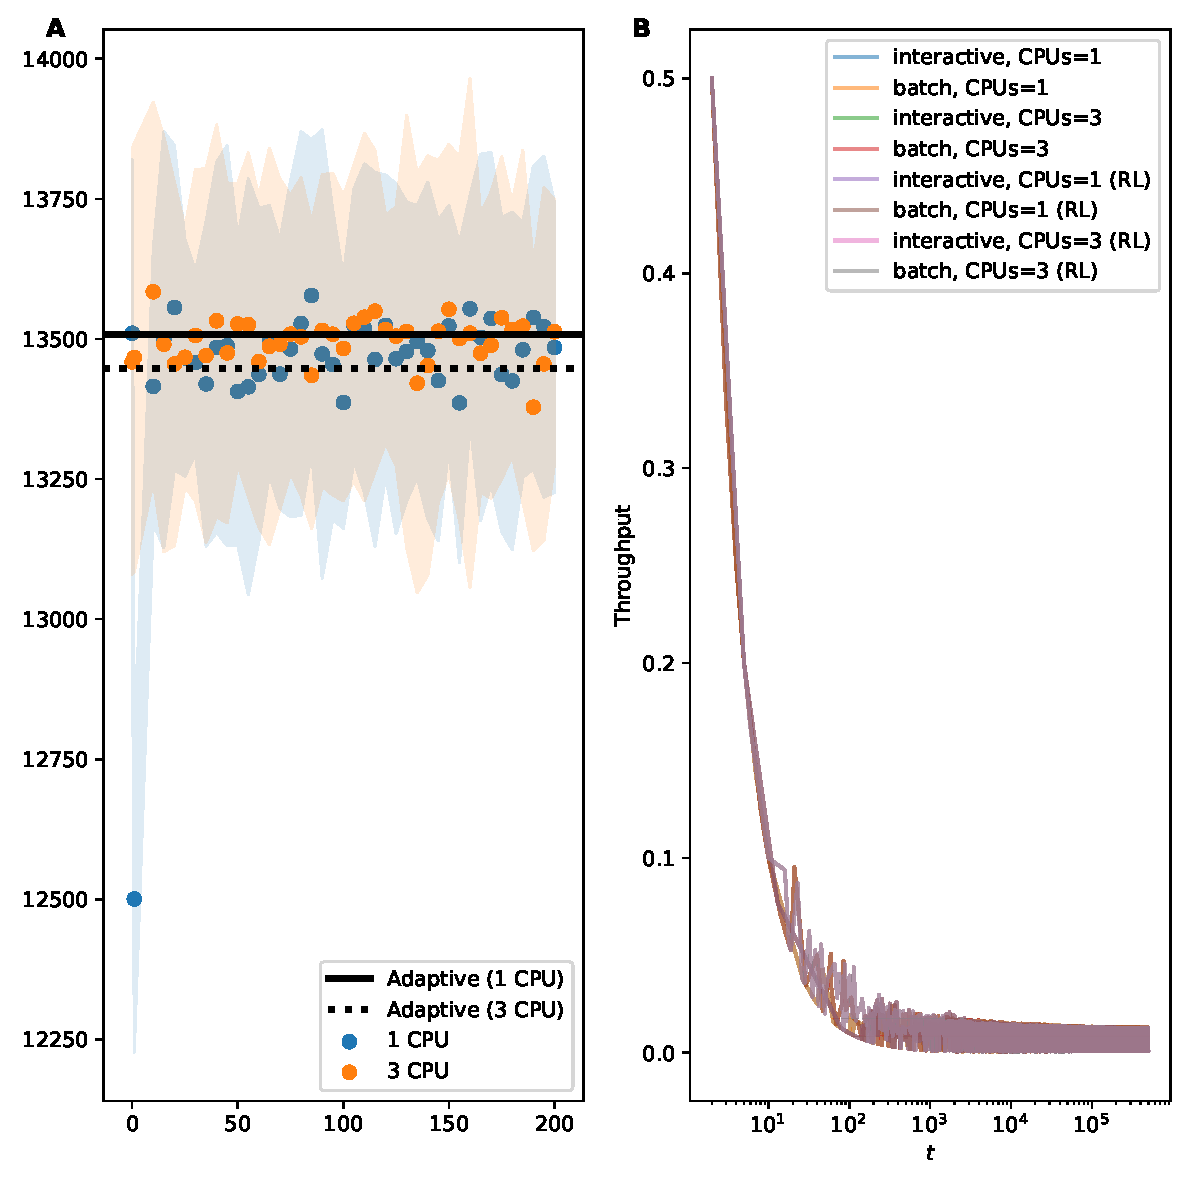
\includegraphics[width=0.75\textwidth]{figs/procs_completed.pdf}
    \caption{Average number of processes completed (\textbf{A}) in the constant and adaptive quantum scheduling
             schema; the shaded region shows the 95\% confidence interval. (\textbf{B}) throughputs per process
             over time.}
    \label{fig:procs_completed}
\end{figure}
%---------------------------------------------------------------------------------------
\section*{Discussion}
Here we have described and provided profiling results of a discrete event simulation of an operating system.
This software model was used to show that, with sufficient effort and time, adaptive preemption may
present promising results in the future of CPU scheduling. Although the adaptive preemptor did not 
outperform round robin, there is an argument that this groundwork could lead to future, more in depth analyses
and practices that may render a more performant agent.
That being said, optimization at this level is key and providing a software hook that infers optimal quanta could 
hinder the system by creating unnecessary CPU overhead.
\par
Although the software bounded limitations of the adaptive preemptor are notable, the adaptive preemption framework
does provide a security measure. Since machine learning solutions are black box algorithms, it is hard to infer from
simple observation the methodology or computation that the agent applies to return the optimal quantum. Given the
recent notion of microarchitectural exploits such as Meltdown and Spectre, methods that rely on iterative observance
of system behavior, RL based preemption could provide a safeguard from these exploits.
%---------------------------------------------------------------------------------------
\section*{Future Work}
This system can be extended in various ways, from increasing the state feature vector size of the
adaptive preemptor or invoking more complex AI machinery for higher accuracy to incorporating
real process behavior data to better approximate OS behavior. Another direction for the work
is to build up a set of realistic subsystems that would themselves contain discrete events in
order to simulate driver interfacing behaviors.
%---------------------------------------------------------------------------------------
\end{document}
